\documentclass[a4paper, 12pt]{article}
\author{Justin Clough, RIN:661682899}
\title{FEP: Assignment 2}
\usepackage[margin=0.75in]{geometry}
\usepackage{float}
\usepackage{enumerate}
\usepackage{listings}
\usepackage{amsmath}
\usepackage{xcolor}
\lstset{
    frame=single,
    breaklines=true,
}
\usepackage{graphicx}
\graphicspath{ {images/} }

\begin{document}
\maketitle

\section*{Algorithm Description}

The reordering algorithm has two main steps, not including
loading or writing the mesh. The first step was to find a starting 
vertex. The second step was to then use the reverse Cuthill-McKee 
algorithm to reorder the mesh nodes. 

The starting mesh vertex was found by first using reverse classification 
to create a list of mesh vertices classified on model vertices. 
This list of mesh vertices was then iterated over twice. 
The first iteration determined the average spatial coordinates of the 
mesh vertices. The second iteration determined which mesh vertex was 
furthest away from this average point. The mesh vertex with the greatest
distance from the center was then used as the starting vertex. A better
alternative would have been to use graph traversal. This would 
instead find the maximum length of the minimum paths 
between mesh verteces.  Either of the vertices at the 
ends of this path could then be used as a starting vertex for the 
reverse Cuthill-McKee algorithm. 

The reverse Cuthill-McKee started by entering a given staring node
into a queue. The queue had three functions to be used when passed a 
mesh entity:
\begin{enumerate}
  \item \emph{put\_back()} which placed items in the queue if 
          a copy of it was not already in the queue and 
          it was not already numbered
  \item \emph{drop\_front()} which returned and removed the 
          front-most item in the queue
  \item \emph{visited()} which returned \emph{true} if the item was
          already in the queue or has been numbered
\end{enumerate}
While the queue was not empty, the first item was removed and numbered.
The numbering started with the the total number of nodes on the mesh
and was decremented each time a node was numbered. If the node 
corresponded to a mesh vertex, then the adjacent mesh edges were
collected. These edges were then iterated over. For each edge, the
adjacent mesh faces were collected. The mesh faces were then iterated
over; they were numbered if they were not numbered already. While 
iterating over the adjacent edges, the vertex on the opposite 
side of the edge was collected and temporarily stored in another queue
if it was not already numbered. Additionally, if mesh nodes 
corresponded to edges and the edge was not already numbered, then it 
was added to the temporary queue. After all adjacent edges were iterated
over, the temporary queue was added to the main queue. 

Figures of the mesh both before and after reordering are shown
in Figures \ref{fig_oa} through \ref{fig_rc}. The code 
begins on page \pageref{sec:code}.
\emph{Before} and \emph{After} reordering images are shown on the
same page for clarity. 

\newpage 

\begin{figure}[H]
  \centering
  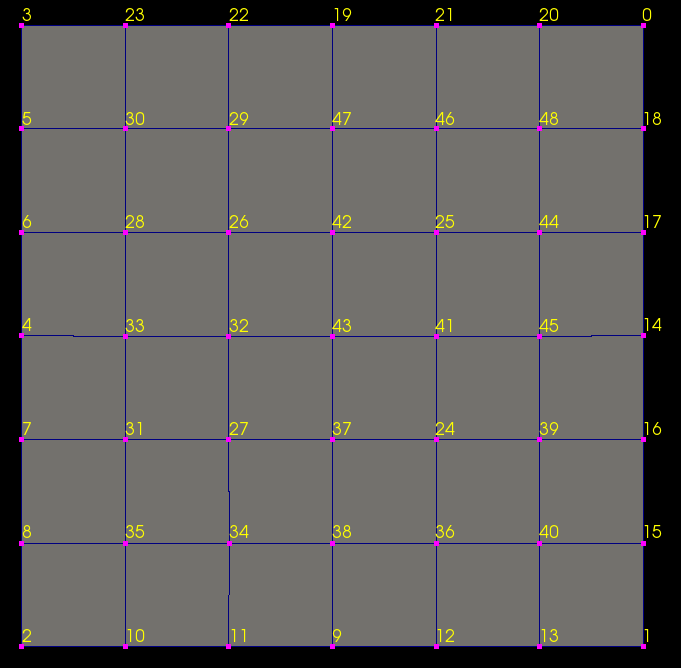
\includegraphics[width=11cm, height=11cm]{orig_a} 
  \caption{Original Numbering for Mesh A. }
  \label{fig_oa}
\end{figure}

\begin{figure}[H]
  \centering
  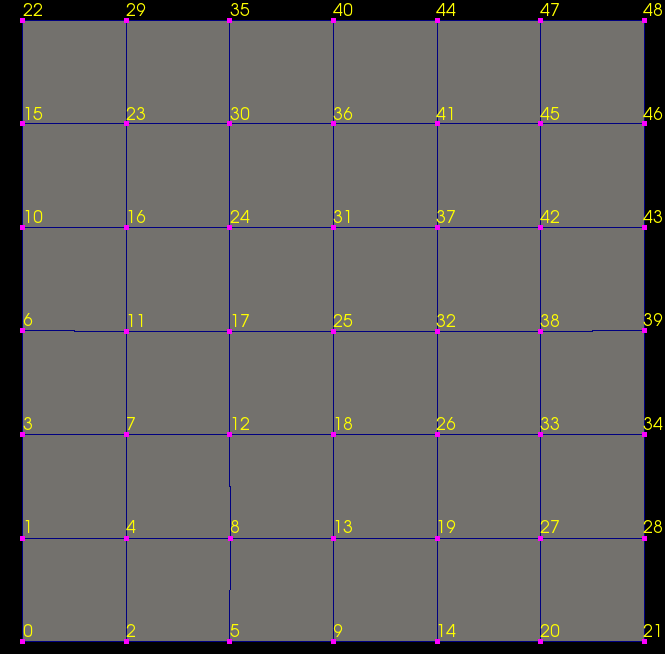
\includegraphics[width=11cm, height=11cm]{reorder_a} 
  \caption{Reorded Numbering for Mesh A. }
  \label{fig_ra}
\end{figure}

\begin{figure}[H]
  \centering
  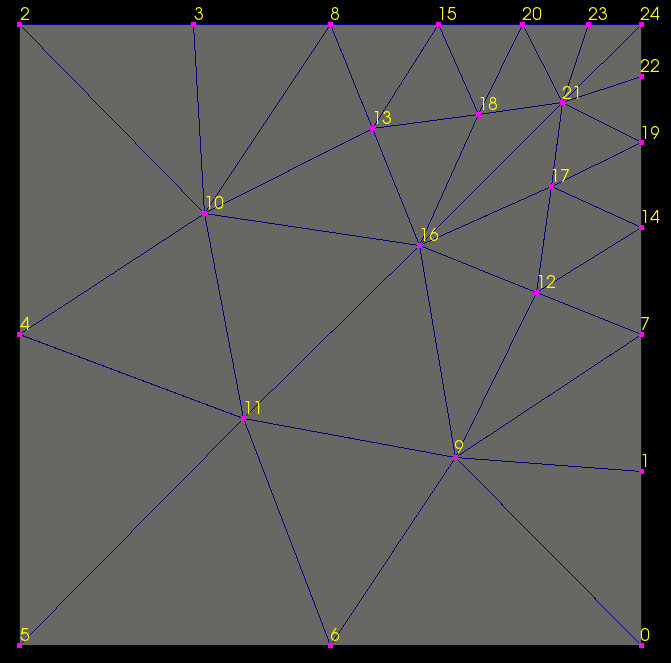
\includegraphics[width=11cm, height=11cm]{orig_b}
  \caption{Original Numbering for Mesh B. }
  \label{fig_ob}
\end{figure}

\begin{figure}[H]
  \centering
  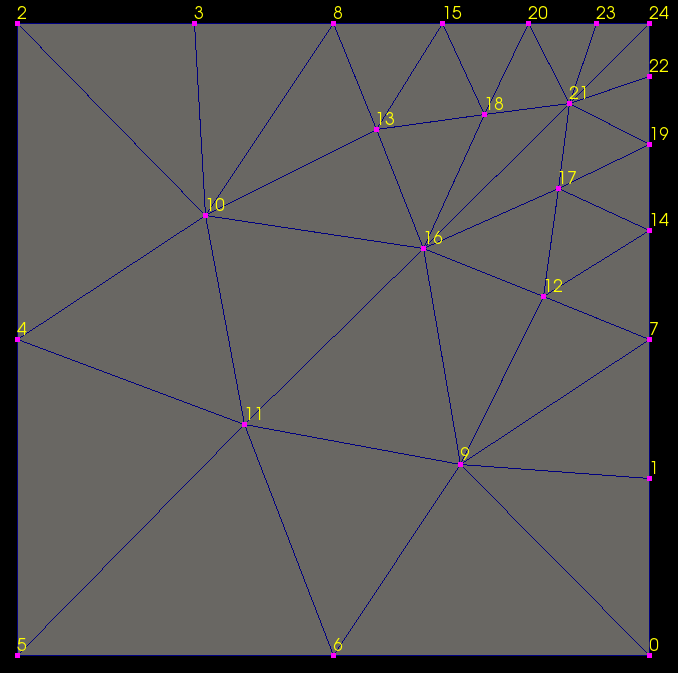
\includegraphics[width=11cm, height=11cm]{reorder_b} 
  \caption{Reorded Numbering for Mesh B. }
  \label{fig_rb}
\end{figure}

\begin{figure}[H]
  \centering
  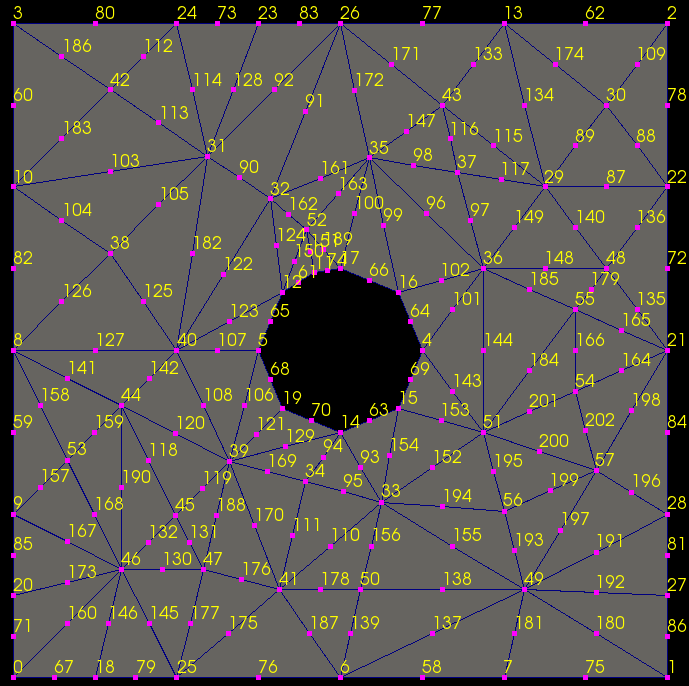
\includegraphics[width=11cm, height=11cm]{orig_c}
  \caption{Original Numbering for Mesh C. }
  \label{fig_oc}
\end{figure}

\begin{figure}[H]
  \centering
  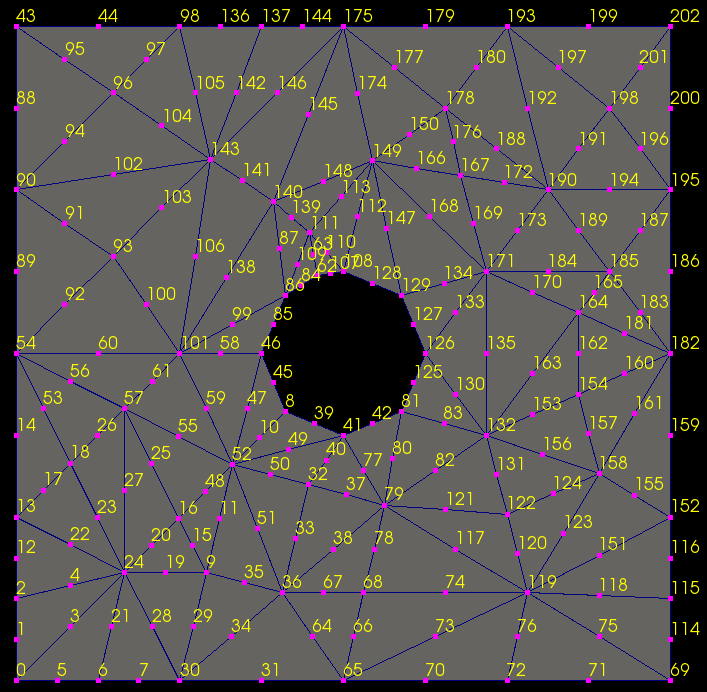
\includegraphics[width=11cm, height=11cm]{reorder_c} 
  \caption{Reorded Numbering for Mesh C. }
  \label{fig_rc}
\end{figure}

\newpage
\section*{Code} \label{sec:code}
\lstinputlisting{/lore/clougj/FiniteElementProgramming/a2/a2.cc}

\end{document}
